\documentclass[10pt]{amsart}
\usepackage[margin=1.4in]{geometry}
\usepackage[usenames,dvipsnames,cmyk]{xcolor} %load first
\usepackage{cancel}
\usepackage{graphicx,subfig}
\graphicspath{ {./images/} }

\usepackage{amssymb,amsmath,enumitem,url}

\newcommand{\D}{\mathrm{d}}
\newcommand{\I}{\mathrm{i}}
\DeclareMathOperator{\sech}{sech}
% \DeclareMathOperator{\cot}{cot}
\DeclareMathOperator{\E}{e}
\DeclareMathOperator{\OO}{O}
\DeclareMathOperator{\oo}{o}
\DeclareMathOperator{\erfc}{erfc}
\DeclareMathOperator{\real}{Re}
\DeclareMathOperator{\imag}{Im}
\usepackage{tikz}
\usepackage[framemethod=tikz]{mdframed}
\theoremstyle{nonumberplain}

\mdtheorem[innertopmargin=-5pt]{sol}{Solution}
%\newmdtheoremenv[innertopmargin=-5pt]{sol}{Solution}
\definecolor{MichiganBlue}{HTML}{00274C}
\definecolor{MichiganYellow}{HTML}{FFCB05}  
\definecolor{NicePurple}{RGB}{75,56,76} %PrincePurple
\definecolor{NiceRed}{RGB}{230,37,52}
\definecolor{MidnightBlue}{rgb}{0.1, 0.1, 0.44}
\usepackage[colorlinks=true, linkcolor=MidnightBlue, citecolor=MidnightBlue, urlcolor=MidnightBlue]{hyperref}

\begin{document}
\pagestyle{empty}

\newcommand{\mline}{\vspace{.2in}\hrule\vspace{.2in}}

\noindent
\text{Hunter Lybbert} \\
\text{Student ID: 2426454} \\
\text{10-14-24} \\
\text{AMATH 567} \\

\title{\bf { Homework 3} }


\maketitle
\noindent
Collaborators*: Laura Thomas, Erin Szalda-Petree, Christina Giannella-Nicolaides, Tomáš Ševček \\
\\
\tiny
\text{*Listed in no particular order. And anyone I discussed at least part of one problem with is considered a collaborator.}
\normalsize
\mline
\begin{enumerate}[label={\bf {\arabic*}:}]
\item From A\&F: 2.2.4. \\
Let $\alpha$ be a real number.
Show that the set of all values of the multivalued function $\log(z^\alpha)$ is not necessarily the same as that of $\alpha \log z$. \\
\textit{Solution:} \\
Let's begin by looking at a precise counter example.
Note when we use the $\log(z)$ we are taking the principal branch where $\theta \in [-\pi, \pi)$.
Let $\alpha = 3$ and $z = i = \E^{i\frac{\pi}{2}}$, then 
\begin{align*}
\alpha \log z &=  3 \log \left( \E^{i\frac{\pi}{2}} \right) \\
&= \frac{3 i \pi}{2}.
\end{align*}
Additionally,
\begin{align*}
\log z^\alpha &=  \log \left( (\E^{i\frac{\pi}{2}})^3 \right) \\
		    &=  \log \left(\E^{i\frac{3\pi}{2}}\right).
\end{align*}
Since $\frac{3\pi}{2}$ is not in our admissible range for $\theta$ we need to adjust it.
Now 
$$
\E^{i\frac{3\pi}{2}} = \E^{i\left(\frac{3\pi}{2} + 2\pi k\right)} =  \E^{-i\frac{\pi}{2}},
$$
where $k \in \mathbb{Z}$ and then taken specifically to be $k=-1$.
Now plugging this back into our calculation of our specific $\log z^\alpha$ we see
$$
\log z^\alpha = \log \left(\E^{i\frac{3\pi}{2}}\right) = \log \left(\E^{-i\frac{\pi}{2}}\right) = -i\frac{\pi}{2} \neq \frac{3 i \pi}{2} = \alpha \log z
$$
Therefore, the values of $\log \left(z^\alpha\right)$ are not necessarily the same as that of $\alpha \log z$.
\qed \\
\item Describe the Riemann surface on which the multi-valued function
  $w(z)$, defined by $w^2=\prod_{j=1}^{n=3}\left(z-a_j\right)$ is
  single-valued. What happens for $n=4,5$ ? For $n>5$ ? You may assume
  that all the $a_j$ are distinct.\\
\textit{Solution:} \\
Before describing the Reimann Surfaces for these cases, I want to establish how I am interpreting $()^\frac{1}{2}$ in the context of this problem.
I am choosing the principal branch for the function $()^\frac{1}{2}$ such that $$\left((z - a_j)(z - a_i)\right)^\frac{1}{2} = (z - a_j)^\frac{1}{2}(z - a_i)^\frac{1}{2}.$$
The branch cut will once again limit the values of $\theta$ to the interval $[-\pi, \pi)$.
Any time we have multiple branch points we need first inspect if any of the branch cuts overlap.
We have to be very careful about the behavior of overlapping branch cuts.
For simplicity, we are taking all branch cuts to be from the branch point $a_j$ going to the left (such that it is the complex number where the $\Re z < \Re a_j$ that is the branch cut which binds $\theta \in [-\pi, \pi)$.
Additionally we add a bit of notation to aid in our discussion of overlapping branch cuts. We write $f(z) = \prod_{j=1}^{n=3}\left(z-a_j\right)$ which can be broken down into components
\begin{align*}
f(z) &= \left(\prod_{j=1}^{n}\left(z-a_j\right)\right)^\frac{1}{2} \\
      &= \prod_{j=1}^{n}\left(z-a_j\right)^\frac{1}{2} \\
      &= (z - a_1)^\frac{1}{2}(z - a_2)^\frac{1}{2}...(z - a_n)^\frac{1}{2} \\
      &= f_1(z)f_2(z)...f_n(z),
\end{align*}
where the second and third lines are equal due to our choice of branch cut as stated at the start of the problem.
Now we need to draw a few pictures and go through a few cases.
Let's begin with the case where $n = 3$ where we have $f(z) = f_1(z)f_2(z)f_3(z)$.
\begin{figure}[h]
	\centering
	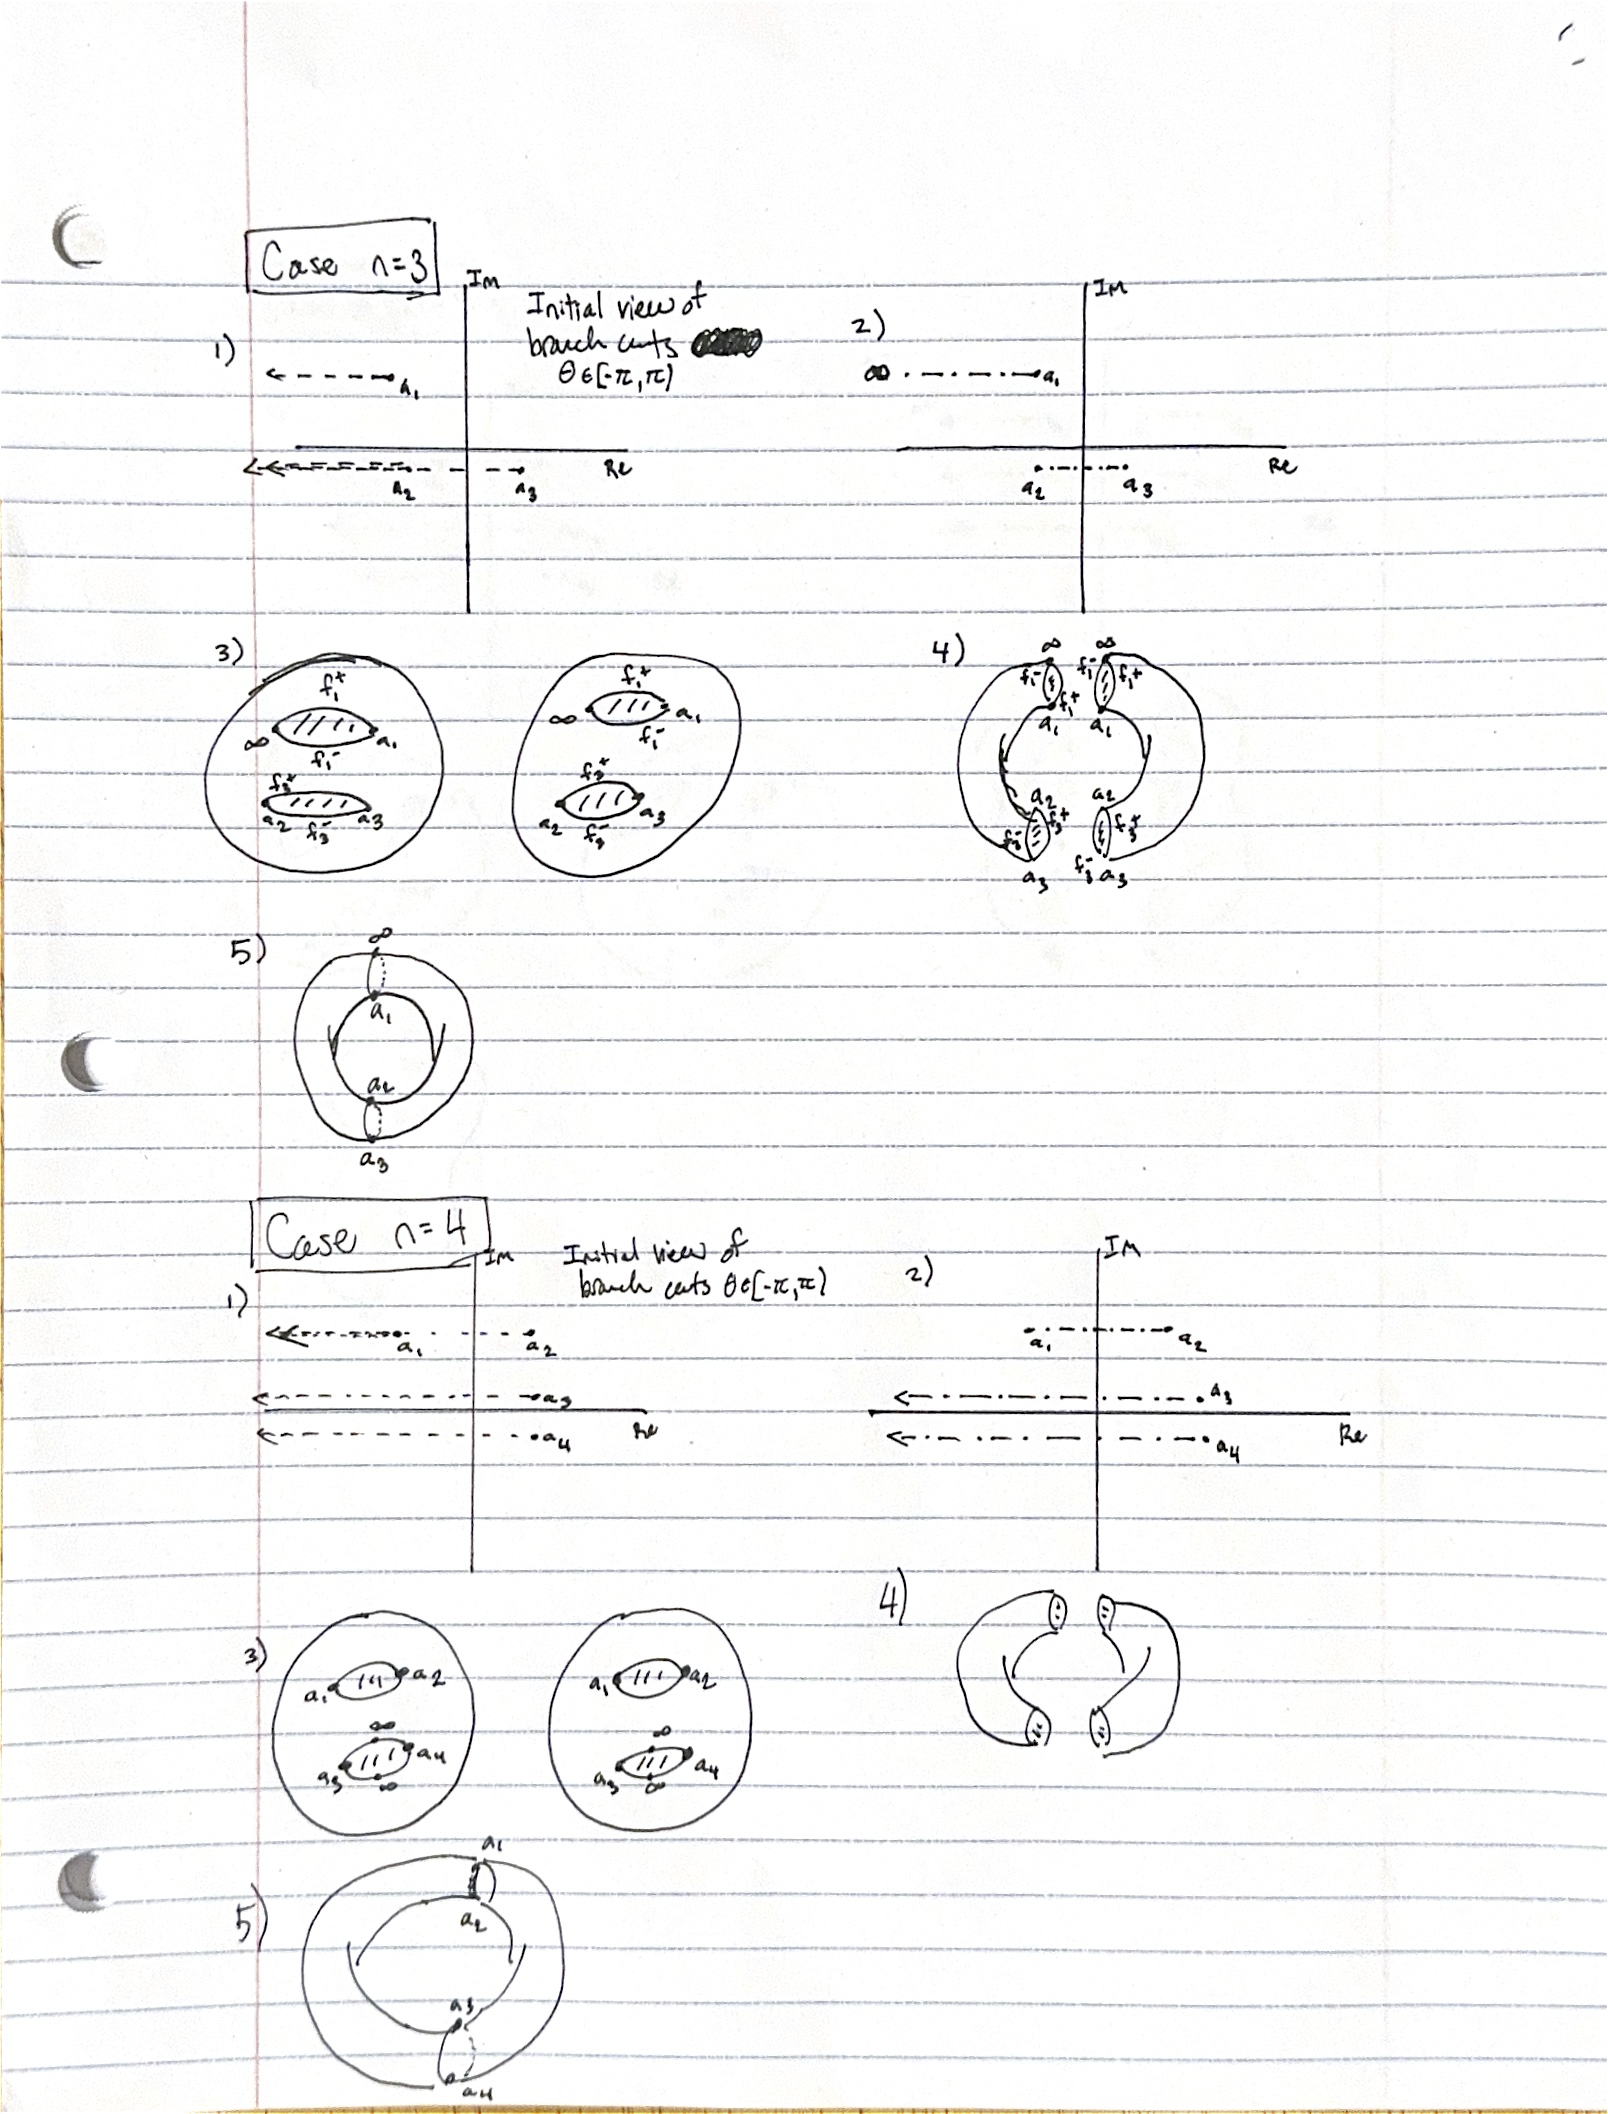
\includegraphics[width=1\textwidth]{riemann_surface_3_4}
 	\caption{
	From problem 2, Riemann Surface drawings where $n=3$ and $n=4$.}\label{fig:f2}
\end{figure}
Now looking at Figure \ref{fig:f2}, I have drawn a feasible Riemann surface step by step.
In step 1) I represent each of the branch cuts starting at the branch points for each $f_1$, $f_2$, and $f_3$.
Notice that $a_2$ and $a_3$ happen to be such that $\Re a_2 = \Re a_3$ therefore their branch cuts overlap from $(-\infty, a_2]$.
Now we investigate the behavior of overlapping branch cuts.
The branch cut for $a_2$ corresponds to where the sign of $f_2$ flips, similarly for $f_3$'s sign flipping.
Notice if the branch cuts overlap, then both $f_2$ and $f_3$'s signs will flip from $+$ to $-$ at the same time.
Notice
$$
f_2f_3 = (-f_2)(-f_3)
$$
therefore overlapping branch cuts actually can cancel on another out.
However, also observe (as a preview to the example I give when $n=5$ in Figure \ref{fig:f3})
$$
f_1f_2f_3 \neq (-f_1)(-f_2)(-f_3) = -f_1f_2f_3.
$$
Therefore, we have that an even number of overlapping branch cuts cancel one another out, but an odd number of overlapping branch cuts is indeed still a branch cut.
I will proceed to carefully describe the $n=3$ case, however these principles can easily be applied and understood as one inspects the drawings for the $n=4$ and $n=5$ cases.
Now returning to our specific scenario drawn for $n=3$, applying what we have established for overlapping branch cuts, the $a_3$ branch cut cancels out the whole $a_2$ branch cut and only leaves the section of the $a_3$ branch cut from $a_3$ to $a_2$ (as depicted in part 2 of Figure \ref{fig:f2}).
Additionally we have a branch cut from $a_1$ to $-\infty$ which evidently is the same as $\infty$ in the complex plane (Riemann Sphere). \\

Now steps, 3-5 of Figure \ref{fig:f2}, proceed through the process of "stretching" these branch cuts apart in two copies of the complex sphere and lining them up appropriately with one another to form a Riemann Surface of a donut shape.
The number of connections between these two copies of the complex sphere depends on the number of branch cuts that remain in the complex domain after we have worked out the overlapping cases.
In Figure \ref{fig:f3} I have depicted the scenario when $n=5$ and $a_1$, $a_2$, $a_3$, $a_4$, $a_5$ happen to be dispersed in the complex plane such that we are left with 3 branch cuts.
Therefore there are 3 places to line up the stretched branch cuts in the complex sphere.
The resulting Riemann Surface in such a scenario is the depicted double torus.
These are the types of Riemann Surfaces which result from a function such as $f(z) = \left(\prod_{j=1}^{n}\left(z-a_j\right)\right)^\frac{1}{2}$.
\qed \\

\begin{figure}[h]
	\centering
	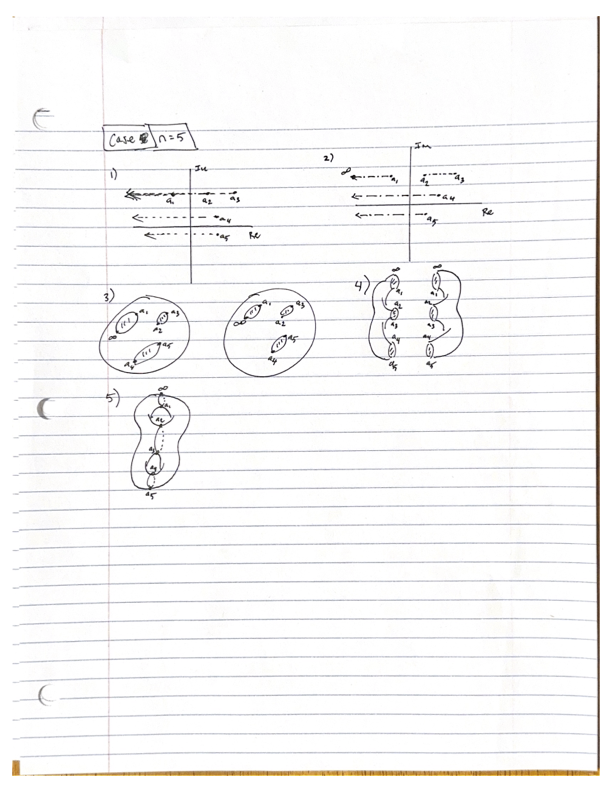
\includegraphics[width=1\textwidth]{riemann_surface_5}
 	\caption{
	From problem 2, Riemann Surface drawings where $n=5$.}\label{fig:f3}
\end{figure}

\item From A\&F: 2.2.5a. \\
Derive the following formulae: \\
a) $$\coth^{-1}(z) = \frac{1}{2}\log\frac{z + 1}{z - 1}$$
\textit{Solution:} \\
We begin with solving for $w$ in $z = \coth{w}$ with $w, z \in \mathbb{C}$. 
\begin{eqnarray*}
z = \coth{w} &=& \frac{\cosh w}{\sinh w} = \frac{ \frac{e^{w} + e^{-w}}{\cancel{2}} }{ \frac{e^{w} - e^{-w}}{\cancel{2}} } = \frac{ e^{w} + e^{-w} }{ e^{w} - e^{-w} } \\
	  &=& \frac{e^{w}}{e^{w}} \frac{ e^{w} + e^{-w} }{ e^{w} - e^{-w} } = \frac{ e^{2w} + 1}{ e^{2w} - 1 }
\end{eqnarray*}
Now let's proceed by multiplying both sides by the denominator
\begin{eqnarray*}
z\left( e^{2w} - 1\right) &=&  e^{2w} + 1\\
ze^{2w} - z &=&  e^{2w} + 1\\
ze^{2w} - e^{2w} &=& z + 1\\
e^{2w}(z - 1) &=& z + 1\\
e^{2w} &=& \frac{z + 1}{z - 1 }\\
\log \left(e^{2w}\right) &=& \log \left(\frac{z + 1}{z - 1} \right) + 2i\pi k, \: k \in \mathbb{Z} \\ \\
2w &=& \log \left(\frac{z + 1}{z - 1} \right) + 2i\pi k, \: k \in \mathbb{Z} \\ \\
w &=& \frac{1}{2}\log \left(\frac{z + 1}{z - 1} \right) + i\pi k, \: k \in \mathbb{Z} \\
\end{eqnarray*}
This is to show
$$\coth^{-1}(z) = \operatorname{arccot}(\coth w) = w = \frac{1}{2}\log \left(\frac{z + 1}{z - 1} \right) + i\pi k, \: k \in \mathbb{Z}.$$
More directly we have 
$$\coth^{-1}(z) = \frac{1}{2}\log \left(\frac{z + 1}{z - 1} \right).$$
as required.
Where the final statement comes from choosing the principal branch of the $\log$, meaning $\theta \in [-\pi, \pi)$.
We also take $k = 0$.
\qed \\
\\
While you're at it, also derive a formula for $\operatorname{arccot}(z)$ in terms of the logarithm. \\
\textit{Solution:} \\
Let's begin by solving for $w$ in this equation $z = \cot w$ with $w, z \in \mathbb{C}$.
\begin{eqnarray*}
z = \cot w &=& \frac{\cos w}{\sin w} = \frac{ \frac{e^{iw} + e^{-iw}}{\cancel{2}} }{ \frac{e^{iw} - e^{-iw}}{\cancel{2}i} } = \frac{ i\left(e^{iw} + e^{-iw} \right)}{ e^{iw} - e^{-iw} } \\
	  &=& \frac{e^{iw}}{e^{iw}} \frac{ i\left(e^{iw} + e^{-iw} \right)}{ e^{iw} - e^{-iw} } = \frac{ i\left(e^{2iw} + 1 \right)}{ e^{2iw} - 1 }
\end{eqnarray*}
Now let's proceed by multiplying both sides by the denominator
\begin{eqnarray*}
z(e^{2iw} - 1) &=& i\left(e^{2iw} + 1 \right) \\
ze^{2iw} - z &=& ie^{2iw} + i \\
ze^{2iw} - z - ie^{2iw} - i &=& 0 \\
e^{2iw}(z - i) &=& z + i \\ 
e^{2iw} &=& \frac{z + i}{z - i} \\
\log \left(e^{2iw}\right) &=& \log \left(\frac{z + i}{z - i} \right) + 2i\pi k, \: k \in \mathbb{Z} \\ \\
2iw &=& \log \left(\frac{z + i}{z - i} \right) + 2i\pi k, \: k \in \mathbb{Z} \\
w &=& \frac{1}{2i}\log \left(\frac{z + i}{z - i} \right) + \pi k, \: k \in \mathbb{Z} \\
\end{eqnarray*}
This is to show
$$\operatorname{arccot}(z) = \operatorname{arccot}(\cot w) = w = \frac{1}{2i}\log \left(\frac{z + i}{z - i} \right) + \pi k, \: k \in \mathbb{Z}.$$
More directly we have 
$$ \operatorname{arccot}(z) = \frac{1}{2i}\log \left(\frac{z + i}{z - i} \right) + \pi k, \: k \in \mathbb{Z}$$
as required. 
Where the final statement comes from choosing the principal branch of the $\log$, meaning $\theta \in [-\pi, \pi)$.
We also take $k = 0$.
\qed
\\

\item Let
  \begin{align*}
    s(z) = z^{1/2} = \rho^{1/2} \E^{\I \theta/2}, \quad \theta \in [-\pi,\pi),
  \end{align*}
  denote the principal branch of the square root.  Show that the
  functions
  \begin{align*}
    f_1(z) = s(z^2 -1), \quad f_2(z) = s(z-1) s(z+1),
  \end{align*}
  are not equal as functions on $\mathbb C$ --- first produce plots and then use a mathematical argument.  Determine the branch cut for $f_2(z)$ (Note: My
  cartoon of what the branch cut for $f_1$ looks like in lecture was
  not accurate).  Find the relationship between $f_1(z)$ and $f_2(z)$.\\
\textit{Solution:} \\
\begin{figure}[h]
	\centering
	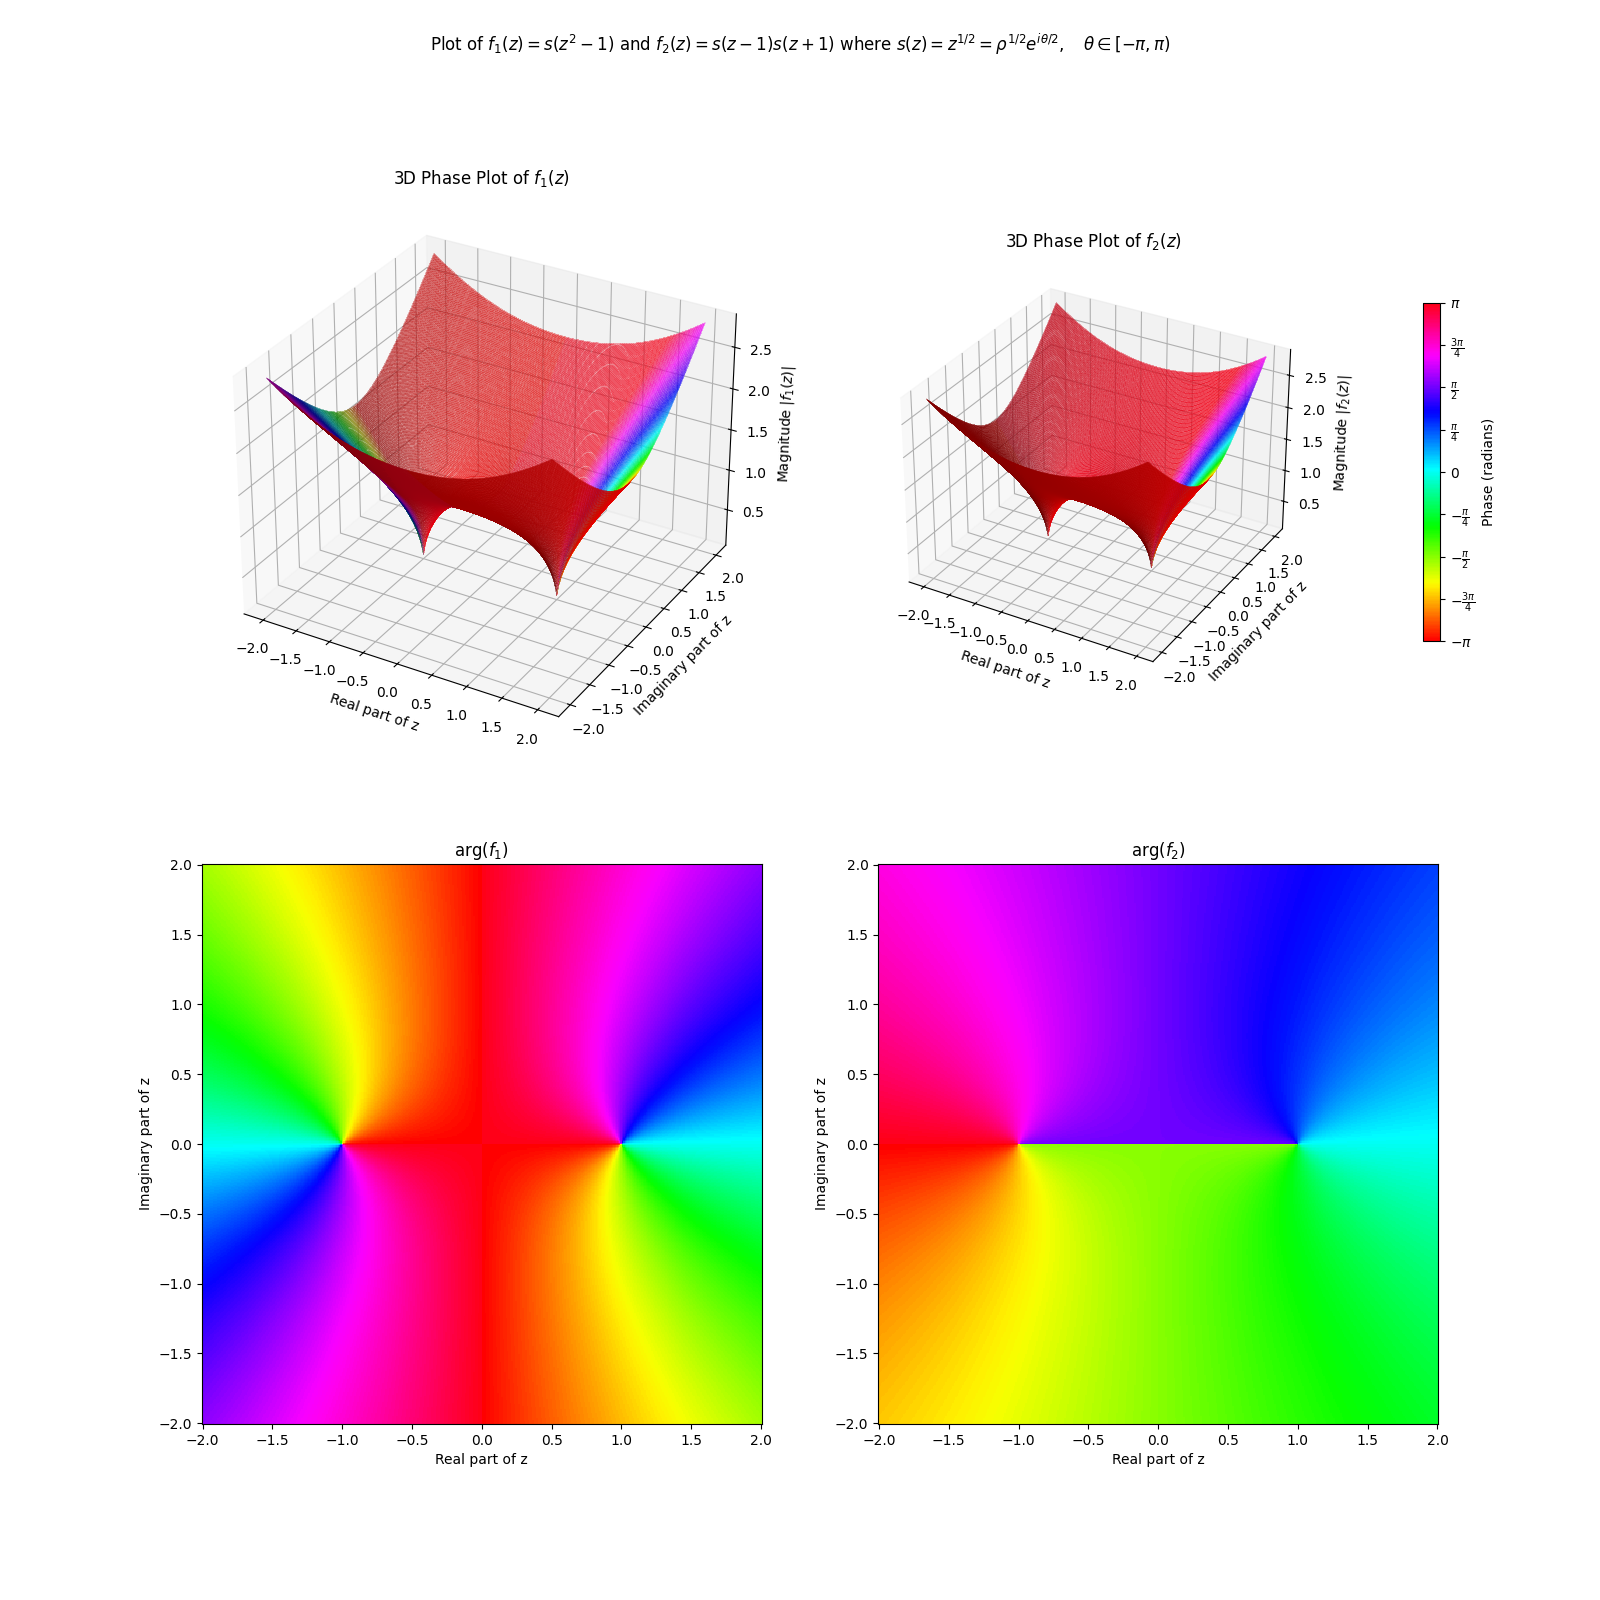
\includegraphics[width=1\textwidth]{problem_4_vis.png}
 	\caption{
	From problem 4, plot lot $f_1(z) = s(z^2 -1)$, $f_2(z) = s(z-1) s(z+1)$, where $s(z) = z^{1/2} = \rho^{1/2} \E^{\I \theta/2},\:\:
	\theta \in [-\pi,\pi)$, denote the principal branch of the square root.}\label{fig:f1}
\end{figure}
\noindent
Notice in Figure \ref{fig:f1} we have two scenarios.
One scenario we are plotting $f_1$ on the left two plots and then $f_2$ in the right plots.
With $f_1$, we see a branch cut both between $-1$ and $1$ along the real axis as well as along the whole imaginary axis where $z$ is purely imaginary.
However, on the $f_2$ plots we only see the branch cut between $-1$ and $1$ along the real axis.
The shabby matplotlib plot appears to indicate there is still a branch cut from $-1$ to $-\infty$, however, as established in problem 2, when an even number of branch cuts overlap their sign switching cancels out resulting in no branch cut in that location.
Now for a more mathematical argument or evidence that these functions are not the same as one another.
Consider if we plug in $z = -2$ to both $f_1$ and $f_2$ \\
\begin{align*}
f_1(-2) &= s((-2)^2 - 1) = s(4 - 1) = (3)^{1/2} = \sqrt{3} \\
f_2(-2) &= s(-2 - 1)s(-2 + 1) = s(-3)s(-1) = \sqrt{-3}\sqrt{-1} = i\cdot i \sqrt{3} = -\sqrt{3}
\end{align*} \\
Therefore, $f_1(z)$ and $f_2(z)$ are not equal as functions on $\mathbb{C}$.
The relationship between $f_1(z)$ and $f_2(z)$ is that they can be equal given certain choice of branch cuts.
However, closely looking at these two functions brings to realize the importance of order of operations in a complex valued function.
Essentially the difference between these functions is $f_1(z)$ performs a multiplication prior to taking the square root while $f_2(z)$ distributes the square root to the factors and performs the square root calculation first before the multiplication between the two parts. It is very interesting how differently these functions behave as complex valued functions.
\qed
\\

  \item Consider the function
    \begin{align*}
     \psi(z) = \int_1^z \frac{\D w}{(w^2 - 1)^{1/2}}, \quad z \not \in
      (-\infty, 1),
    \end{align*}
    where the path of integration is a straight line from $1$ to $z$.
    \begin{itemize}
   \item  Show that
    \begin{align*}
      \psi(z) = \log \varphi(z), \quad \varphi(z) = z + (z^2 -
      1)^{1/2}, \quad z \not \in
      (-\infty, 1),
    \end{align*}
   for an appropriate choice of branch cut for $(z^2 -
   1)^{1/2}$.  Here $\log z$ denotes the principal branch. \\
   \textit{Solution:} \\
   We will first show that $\log \varphi(z)$ is analytic.
   Showing that this function satisfies the Cauchy-Riemann equations or showing the formal definition of the derivative in terms of the $\lim$ is difficult. 
   Rather, we will show $\log \varphi(z)$ is composed of analytic functions, given the correct choices of branches, where necessary.
   First, we choose the branch cut of $(z^2 - 1)^{1/2}$ s.t. it is equal to $(z - 1)^{1/2} (z + 1)^{1/2}$ and we limit $\theta \in [-\pi, \pi)$.
   Now we have \\
   $$\varphi(z) = z + (z - 1)^{1/2}(z + 1)^{1/2}$$ \\
   which is analytic away from the real axis between [-1,1]. This is because the sum of analytic functions is analytic (where $z$ is already analytic and $(z - 1)^{1/2}(z + 1)^{1/2}$ is as well because of branch cut choices already discussed). Now, here we take the branch cut for $\log z$ to be along the negative real axis such that $\theta \in [-\pi, \pi)$. If we can show the input to our $\log$ function ($\varphi(z)$) will not be 0 or purely real negative, we will have that $\log(\varphi(z))$ is analytic. The only way $\varphi(z)$ could be 0 is if $z = (z - 1)^{1/2}(z + 1)^{1/2}$. Lets assume by way of contradiction they are equal:
   \begin{align*}
   z &= (z - 1)^{1/2}(z + 1)^{1/2} \\
   z^2 &= (z - 1)(z + 1) \\
   z^2 &= z^2 - 1 \\
   0 &\neq - 1
   \end{align*}
   which is not true therefore our assumption is false, and thus $\varphi(z)$ will never be 0.
   Concerning $\varphi(z)$ being real negative, it will suffice to show that $(z - 1)^{1/2}(z + 1)^{1/2}$ is never real negative (since the our assumption $z \not \in (-\infty, 1)$ guaruntees that what we are adding to that product will not be real negative).
   Now, our choice of branch cut for the square root actually guarantees that $(z - 1)^{1/2}(z + 1)^{1/2}$ will be at least non real negative since we are choosing the branch cut that chooses the principal branch.
   Continuing on, we will show that $\log \varphi(z)$ is indeed the anti-derivative of what we have in the integrand.
   To show that $\log \varphi(z)$ is the anti-derivative of the integrand we begin by taking the derivative of $\log \varphi(z)$.
   \begin{align*}
   \frac{\D}{\D z} \log (z + (z^2 - 1)^{1/2}) &= \frac{1}{(z + (z^2 - 1)^{1/2})}\left( 1 + \frac{1}{2}\frac{2z}{(z^2 - 1)^{1/2}} \right) \\
							     &= \frac{1}{(z + (z^2 - 1)^{1/2})}\left( \frac{(z^2 - 1)^{1/2}}{(z^2 - 1)^{1/2}} + \frac{z}{(z^2 - 1)^{1/2}} \right) \\
							     &= \frac{1}{(z + (z^2 - 1)^{1/2})}\left( \frac{(z^2 - 1)^{1/2} + z}{(z^2 - 1)^{1/2}} \right) \\
							     &= \frac{1}{(z^2 - 1)^{1/2}} \\
   \end{align*}
   Which is the same as our term in the integrand.
   Since, $F(z)$ is analytic in the region we care about $(z)$ and $F^\prime(z) = f(z)$ we can use the FTC to say
   \begin{align*}
   \psi(z) = \int_1^z \frac{\D w}{(w^2 - 1)^{1/2}} &= F(z) - F(1) \\
							&= \log(\varphi(z)) - \log(\varphi(1)) \\
							&= \log(z + (z - 1)^{\frac{1}{2}}(z + 1)^{\frac{1}{2}}) - \log(1 + (1 - 1)^{\frac{1}{2}}(1 + 1)^{\frac{1}{2}}) \\
							&= \log(z + (z - 1)^{\frac{1}{2}}(z + 1)^{\frac{1}{2}}) - \log(1 + (0)^{\frac{1}{2}}(0)^{\frac{1}{2}}) \\
							&= \log(z + (z - 1)^{\frac{1}{2}}(z + 1)^{\frac{1}{2}}) - \log(1) \\
							&= \log(z + (z - 1)^{\frac{1}{2}}(z + 1)^{\frac{1}{2}}) \\
							&= \log(\varphi(z))
   \end{align*}
   Therefore $\psi(z) = \log(\varphi(z))$.
   Technically I should evaluate a limit of $F(1 + \epsilon)$ as $\epsilon \rightarrow 0$ to be allowed to evaluate $F(1)$ in our usage of the FTC, since we had excluded 1 from our admissible input, but I will only come back to this if I have time.
   \item Find an expression for
   \begin{align*}
     \gamma(z) = \int_{-1}^z \frac{\D w}{(w^2 - 1)^{1/2}}, \quad z \not \in
      (-1, \infty),
   \end{align*}
   in terms of $\varphi(z)$ and the principal branch of the logarithm.  Again, the path of integration is a
   straight line. \\
   \textit{Solution:} \\
   We will use a similar argument as in part 1, but this time we need to make slightly different choices of branch cuts to ensure the functions we care about are in analytic in the right regions.
   I am proposing that solution will be \\
   $$
   \gamma(z) = \log(-\varphi(z)).
   $$ \\
   Let's verify all of the same things as we did in part 1.
   That includes the following
   \begin{itemize}
   \item ensure $F^{\prime} = f(z)$
   \item Choose the branch cut such that $\theta \in [0, 2\pi)$ and we exclude the region that is the real positive axis in order to ensure $\log$ is analytic where it needs to be
   \item Choose the right branch cut for $()^\frac{1}{2}$ such that the cut is between [-1, 1]
   \item recall that since we are not allowed to input real positive numbers to the sqrt function it will not put out real positive outputs either.
   \end{itemize}
 \end{itemize}

 \item Show that $\varphi,$ from the previous problem, maps $\mathbb C \setminus [-1,1]$ onto the
   exterior of the unit disk, $\{ z \in \mathbb C ~:~ |z| > 1\}$.
   Furthermore
   \begin{align*}
     \frac 1 2 \left( \varphi(z) + 1/\varphi(z) \right) = z, \quad \mathbb C \setminus [-1,1].
   \end{align*}
\textit{Solution:} \\
We want to show $\varphi(z) = z + \sqrt{z - 1}\sqrt{z + 1}$ maps everything off the real axis from [-1,1] onto the exterior of the unit disk. In other words we want to show that for $z \in \mathbb C \setminus [-1,1]$ we have 
$$
\left| \varphi(z) \right| > 1.
$$
\\
The second statement can be shown as follows \\
\begin{align*}
\frac{1}{2}\left(\varphi(z) + \frac{1}{\varphi(z)}\right) &= \frac{1}{2}\left(\frac{\varphi(z)^2}{\varphi(z)} + \frac{1}{\varphi(z)}\right) \\
   &= \frac{1}{2}\left(\frac{\varphi(z)^2 + 1}{\varphi(z)}\right) \\
   &= \frac{1}{2}\left(\frac{(z + \sqrt{z - 1}\sqrt{z + 1})^2 + 1}{\varphi(z)}\right) \\
   &= \frac{1}{2}\left(\frac{z^2 + 2 z \sqrt{z - 1}\sqrt{z + 1} + (z - 1)(z + 1) + 1}{\varphi(z)}\right) \\
   &= \frac{1}{2}\left(\frac{z^2 + 2 z \sqrt{z - 1}\sqrt{z + 1} + z^2 - 1 + 1}{\varphi(z)}\right) \\
   &= \frac{1}{2}\left(\frac{2z^2 + 2 z \sqrt{z - 1}\sqrt{z + 1}}{\varphi(z)}\right) \\
   &= \frac{2z}{2}\left(\frac{z + \sqrt{z - 1}\sqrt{z + 1}}{\varphi(z)}\right) \\
   &= \frac{2z}{2}\left(\frac{\varphi(z)}{\varphi(z)}\right) \\
   &= z
\end{align*}
\qed
\\

   \item (Sharpness of the Bernstein--Walsh inequality)  The
     Bernstein--Walsh inequality states that if a polynomial $p_n$ of
     degree $n$ satisfies $\max_{-1 \leq x \leq 1} |p_n(x)| \leq 1$
     then
     \begin{align*}
       |p_n(z)| \leq |\varphi(z)|^n, \quad z \in \mathbb C \setminus [-1,1].
     \end{align*}
     Show that
     \begin{align*}
        T_n(z) = \frac 1 2 \left( \varphi(z)^n + \varphi(z)^{-n}
       \right), \quad z \in \mathbb C \setminus [-1,1]
     \end{align*}
     is a polynomial that satisfies
     \begin{align*}
       \max_{-1 \leq x \leq 1} |T_n(x)| &= 1,\\
       \lim_{n \to \infty} |T_n(z)|^{1/n} &= |\varphi(z)|,
     \end{align*}
     for any fixed $z \in \mathbb C \setminus [-1,1]$. \\
\textit{Solution:} \\
\end{enumerate}

\end{document}

%%% Local Variables:
%%% mode: latex
%%% TeX-master: t
%%% End:
